\documentclass[]{article}

\usepackage[pdftex]{graphicx}
\usepackage[top=1in, bottom=1in, right=1.25in, left=1.25in]{geometry}
\usepackage{hyperref}

\begin{document}

	% Title Page
	\begin{titlepage}



		\title{\textbf{Bucknell ProPANE Final Report}}
		\author{BU ProPane Team:\\Griffin Dunn\\Colin Madigan\\Phillip Stahlfeld\\\\Clients:\\Dr. Robert Gabauer\\Dr. Robert Midkiff\\\\Advisor:\\Dr. Matthew Watkins}
		\date{April 29, 2013}
		\maketitle



		
		
		\thispagestyle{empty}
		\noindent
		The goal of this report is to document the major technical aspects of the ProPANE system and the process used to make the major technical decisions. 
		
		
		
	\end{titlepage}
	
	\thispagestyle{empty}
	
	
	% Begin  Real  Document
	\tableofcontents
	\newpage
	
	
	\setcounter{page}{1}
	\thispagestyle{empty}
	
	\section{Project Overview}
		One of the problems that professors at Bucknell University face is that they do not have a record of what was actually presented on whiteboards during their lectures. Despite having every lecture planned out on paper, there is still the problem of when a student asks a question that requires further explanation. The material displayed on the board that is not on a professor's written plan becomes lost once the board is erased. As seen in Figure \ref{fig:cive-notes}, some professors have found ways to keep track of some of this information, but these methods can consume unnecessary portions of class. Professors are not the only ones who require a means for capturing the information displayed on boards. Some students are not capable of taking notes themselves and Bucknell is legally required to provide a means for them to obtain copies of the information presented on boards in class. Currently, the solution to this problem is to assign a note-taker who is responsible for recording information presented on the board and then sending a copy of the notes to the professor so that the notes can be distributed to students who are incapable of taking notes themselves. This places extra stress on the note-taker because the notes have to be copied exactly as from the board (including all of the information, in the proper layout, without shorthand notation, and following the same color scheme). Essentially, both students and professors need a way of capturing all of the information written on whiteboards during lectures. The goal of the Bucknell University Professional Portable Automatic Note Extraction (BU ProPANE) system is to solve this problem by automatically capturing digital images of the information presented on the board and sending the images to professors.\\
		\\
		This project is especially relevant to anyone concerned with learning disabilities because it simplifies the process for assisting students with certain disabilities. For example, according to Dr. Midkiff of Bucknell University, some students have a difficult time reading colored writing on a white background. By applying a red filter to digital images of a whiteboard, the colored writing will be set on a red background and allow the student to read the information. There are numerous other ways that digital image manipulation can make information accessible to students whose disabilities prohibit them from learning the information presented on a whiteboard during a class.\\
		\\
		One of the obvious solutions to this problem is to use SMART boards which are essentially large touch screens, but this would mean that SMART boards would have to be installed in every classroom where a student with learning disabilities has class. The goal of BU ProPANE is to create a portable system that can be used in any classroom with very little setup time. Ideally, this will reduce costs and interfere less with the way professors currently teach classes. 
		
		% Image of Professor Gabauer's lecture notes
		\begin{figure}[h]
      			\centering
      			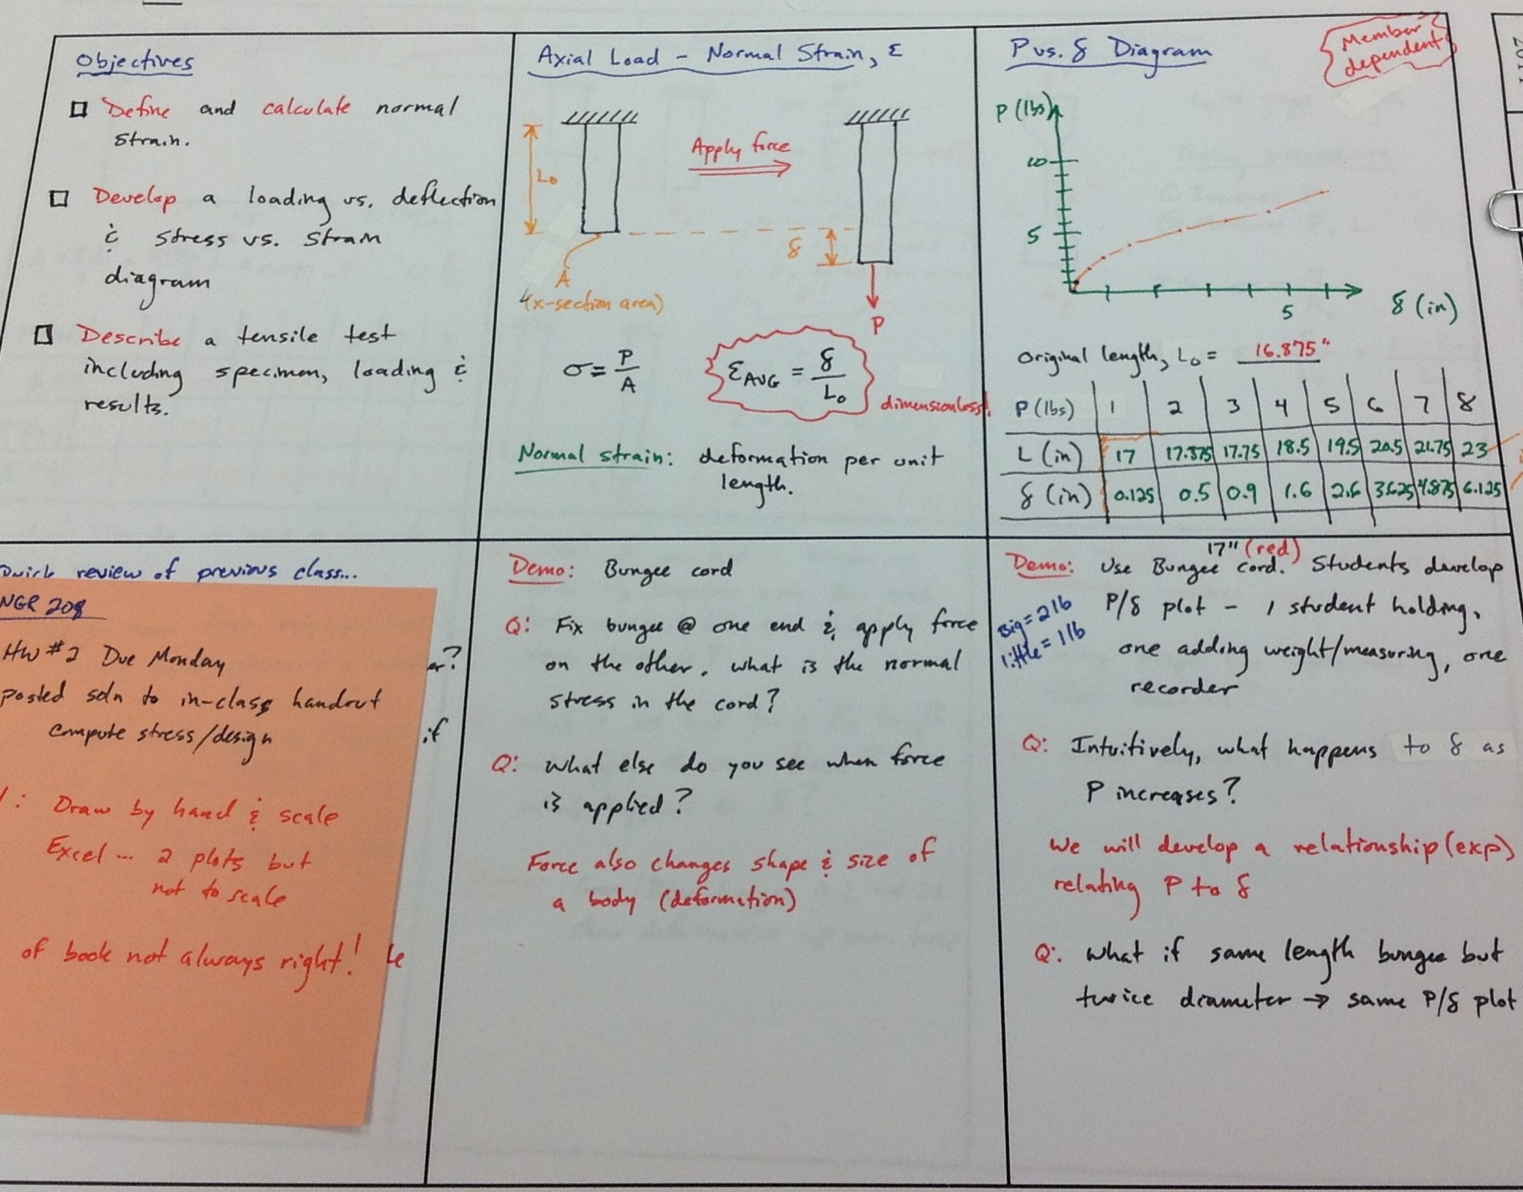
\includegraphics[scale=0.2]{./images/cive-notes.png}
			\caption{Image of civil engineering lecture notes. Orange note is an example of how lecture notes are recorded and altered. Image courtesy of Doug Gabauer 2012.}
			\label{fig:cive-notes}
   		 \end{figure}

	\section{Background}
	\subsection{Signal Processing}

According to the IEEE Signal Processing Society, 
		{\quotation {\sl \noindent Signal processing is the enabling technology for the generation, transformation, and interpretation of information. It comprises the theory, algorithms, architecture, implementation, and applications related to processing information contained in many different formats broadly designated as signals. Signal refers to any abstract, symbolic, or physical manifestation of information with examples that include: audio, music, speech, language, text, image, graphics...  \\
\noindent Signal processing uses mathematical, statistical, computational, heuristic, and/or linguistic representations, formalisms, modeling techniques and algorithms for generating, transforming, transmitting, and learning from analog or digital signals, which may be performed in hardware or software. Signal generation includes sensing, acquisition, extraction, synthesis, rendering, reproduction and display. Signal transformations may involve filtering, recovery, enhancement, translation, detection, and decomposition. The transmission or transfer of information includes coding, compression, securing, detection, and authentication. Learning can involve analysis, estimation, recognition, inference, discovery and/or interpretation.}}  \cite{IEEESPS} \\

\noindent Signal processing applies to both analog and digital signals.  Analog signals are sets of continuous values, and can be directly processed using both linear and non-linear electronic circuits.  These signals can be sampled to obtain a signal with the same values, but only at discrete points over an interval in time.  These signals can also be directly processed with electronic circuitry, but they can also be digitized to create digital signals.  Digital signal processing can be done conveniently on computers, or on dedicated digital circuits such as application-specific integrated circuits (ASICs) and field-programmable gate arrays (FPGAs).  For this project, we are interested in digital signal processing, and specifically the field of image processing. \\

		\subsection{Image Processing}

Digital images are electronic representations of physical media, such as photographs, texts, artwork and more.  The digital image is sampled and mapped as a grid of pixels.  Each pixel is assigned a tonal value (black, white, shades of gray or color) which is represented in binary.  The bits representing each pixel are stored by a computer and can be compressed via mathematical reduction of some kind.  To view an image, the bits are interpreted and read by the computer to produce an analog version for display. \\ 

\begin{figure}[h]
      			\centering
      			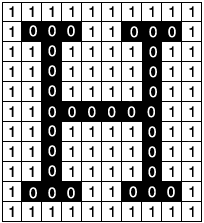
\includegraphics[scale=0.75]{./images/research_image_processing_1}
			\caption{A bitonal image, where each pixel is assigned either a 0 or 1 to represent color.}
			\label{fig:research_image_processing_1}
   		 \end{figure}

\noindent Digital images can be displayed with different resolutions.  Resolution is the ability to display fine spatial detail.  In general, resolution increases with sampling frequency.  Common units of resolution are dots-per-inch (dpi) and pixels-per-inch (ppi).   \\ 

\noindent The number of bits used to define each pixel is defined as the bit depth.  The greater the bit depth, the greater the number of tones can be represented.  Normally, a color image is represented by a bit depth of 8 to 24.  In a 24-bit image, the bits are often divided into red, green and blue, with 8 bits for each color.  Other colors are obtained from combinations of those bits.  In a 24-bit image, there are 16.7 million color values ($2^{24}$).  	\\ 

\noindent To reduce image file size for storage, processing and transmission, compression is used.  Compression techniques use algorithms to abbreviate the binary code in an uncompressed image.  Both lossless and lossy forms of compression exist. Lossless schemes abbreviate the binary code without discarding any information so that the decompressed image is bit-for-bit identical to the original.  Lossy schemes average and discard the least significant information based on an understanding of visual perception.  JPEG is a common lossy compression scheme.  Some lossy-compressed images may appear identical to the raw image, and are considered ``visually lossless''.  \cite{cornell} 

\begin{figure}[h]
      			\centering
      			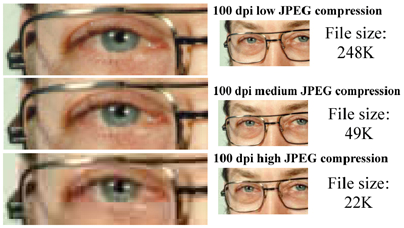
\includegraphics[scale=0.75]{./images/research_image_processing_2}
			\caption{Example of a ``visually lossless'' compressed image.  The full images look the same regardless of compression level, but the zoomed in images get blurrier as compression increases.}
			\label{fig:research_image_processing_2}
   		 \end{figure}

\subsection{Image Processing Tools}

\noindent Image processing can be implemented using a variety of different tools.  There are programs, such as Adobe Photoshop, which provide users with a graphical user interface and on-screen tools to use to edit their images.  While programs like this can achieve desirable high-quality results, the process can be time-consuming for an individual image, and must be repeated for each subsequent image.  A far better option for similar processing of a large quantity of images is to use a programming language with an image processing library.  The user can write a program which performs desired effects on any number of images.  A variety of libraries exist to add image processing features to many programming languages.  The libraries listed in this section are for common programming languages and seem to have some or all of the functionality required for the ProPANE project.  \\ 

\noindent {\sl Eutecus Signal and Image Processing Library} \cite{eutecus} \\

\noindent A collection of general-purpose, optimized C++ routines and classes, along with utility classes to aid image and video file manipulation.  These routines are usually used in computationally intensive real-time applications, where optimal execution speed is critical.  For use, licensing rights must be purchased. \\

\noindent {\sl OpenCV} \cite{opencv} \\

\noindent A free library of programming functions for real time computer vision, originally developed by Intel.  It has interfaces for C, C++, Python, and soon Java, running on Windows, Linux, Android and Mac.  There are over 2500 algorithms optimized for image processing.  \\

\noindent {\sl Aforge.NET Framework} \cite{aforge1} \\

\noindent A free, open-source C\# framework, containing libraries for image processing, robotics, and more.  The image processing library, AForge.Imaging, contains different image processing routines, aimed to help with image enhancement and processing.  \\

\noindent {\sl Python Imaging Library} \cite{pil} \\

\noindent A free library which adds image processing capabilities to the Python interpreter.  It supports many file formats and provides powerful image processing and graphics capabilities. \\

\noindent {\sl VIPS} \cite{vips} \\

\noindent A free image processing system.  Good with large images, with many CPUs.  It needs little memory and runs quickly compared to many libraries.  The library can be used from C, C++, command line, Python, Ruby, JavaScript and others.  Includes a GUI for Photoshop-style editing. Works on Linux/Unix, Windows 7 and MacOS. \\

\noindent {\sl MATLAB Image Processing Toolbox} \cite{matlab_ipt} \\ 

\noindent A comprehensive set of reference-standard algorithms and graphical tools.  For image processing, analysis, visualization, and algorithm development.  Features include image enhancement, deblurring, feature detection, noise reduction, segmentation, geometric transformations, and image registration.  Using the Image Acquisition Toolbox, images can be acquired directly from a camera and read into MATLAB or Simulink. \cite{matlab_iat} \\ 


\noindent {\sl Mathematica} \cite{mathematica} \\

\noindent Mathematica provides built-in support for programmatic modern industrial-strength image processing, fully integrated with its powerful mathematical and algorithmic capabilities.  Mathematica's symbolic architecture and notebook paradigm allow images in visual form to be included and manipulated directly both interactively and in programs.


	\subsection{Image Processing Techniques}

\noindent Many techniques currently exist for processing images in numerous different ways.  The techniques in this section seem relevant to the image processing necessary for the ProPANE system. \cite{ndt} \\ \\
{\sl Image Analysis- \\ \indent Extract information from the image} 
			\begin{itemize} 
				\item{\textbf{Image statistics:}} Calculates the maximum, minimum, average, standard deviation, variance, median, and mean-square intensities of the image data					
				\item{\textbf{Gray-scale mapping:}} Alters the mapping of the intensity of pixels in a file to match the intensity displayed on a computer screen 
				\item{\textbf{Image extraction:}} Extracts a portion or all of an image and creates a new image with the selected area 
				\item{\textbf{Slice:}} Plots intensity versus position for any direction. Lists intensity versus pixel location from any point along the slice
			\end{itemize} 
{\sl Convolution and Noise Filtering- \\ \indent Decrease noise by diminishing statistical deviations}
			\begin{itemize}
				\item{\textbf{High-pass filter:}} Emphasizes regions with rapid intensity changes
				\item{\textbf{Low-pass filter:}} Smooths images, blurs regions with rapid change
				\item{\textbf{Adaptive smoothing filter:}} Sets pixel intensity to a value between original and mean values, corrected by degree of noisiness. Good for decreasing statistical, especiall signal-dependent noise
				\item{\textbf{Median filter:}} Sets pixel intensity to the median intensity of pixels in a neighborhood. Excellent for eliminating intensity spikes
				\item{\textbf{Sigma filter:}} Sets pixel intensity equal to the mean of the intensities in a neighborhood within two of the mean.  Good for signal-independent noise
			\end{itemize}
{\sl Edge Detection- \\ \indent Sharpen intensity-transition regions}	
			\begin{itemize}
				\item{\textbf{First-difference:}} Subtracts intensities of adjacent pixels.  Emphasizes noise as well as desired changes. 
				\item{\textbf{Sobel operator:}} Weighs inner pixels twice as heavily as corner values.  Calculates intensity differences
			\end{itemize}
{\sl Enhancement- }
			\begin{itemize}
				\item{\textbf{Histogram equalization:}} Redistributes the intensities of the image
			\end{itemize}

\subsection{Learning Disabilaties}
        \subsubsection*{Introduction}
One of the major motivating factors behind designing our image capturing system is to help meet the needs of students with disabilities. The term "students with disabilities" is a very broad term, however, so we would like to use the following section to help describe some of the things that mildly disabled students have trouble with at Bucknell, and would therefore need our system to capture information presented on the board for them. \\
Disabilities that students might have that impair their ability to take notes: \cite{disability}
    \begin{itemize}
        \item Visual Impairments
        \begin{itemize}
            \item May be fully blind and need notes translated into Braille
            \item May not see well and need large print letters
            \item May have trouble copying information from whiteboards, projectors, etc.
            \item May have trouble seeing certain colors when framed by a white or black background
        \end{itemize}
        \item Specific Learning Disabilities
        \begin{itemize}
            \item Reading disability
            \item Writing disability
            \item Spelling disability
            \item Inability to copy what they see
            \item Inability to write what they hear
            \item Inability to write legibly
            \item Number reversal problems
        \end{itemize}
        \item Mobility Impairments
        \begin{itemize}
            \item Physically unable to write
            \item Physically unable to write quickly
            \item May be unable to effectively handle a writing implement
        \end{itemize}
        \item Partial or full loss of hearing
    \end{itemize}

\noindent This is just a small portion of the many disabilities faced by students in universities around the world. We hope to help them by giving them full access to all information presented on boards during lectures. By providing easily accessible, easily modifiable images, we hope to help even the playing field for students with disabilities.
Secondary goals of our project will help to make the learning process even easier. Some students get distracted if they see more than one line of text at a time. If we have enough time we will help these students by providing slide bars that will cover portions of the images that students are not currently viewing. This and many other minor features are things that we will accomplish if we have free time after completing our primary objectives. 
		
		
	% Basically just copied tech spec into here	
	\section{Specification}
		The following subsections contain the specifications created in the fall for this project.
		\subsection{Overview}
			The goal of this project is to create a system that captures information written on whiteboards throughout the course of a class. The system should be useable by professors during a standard lecture. The system must be portable so that it can be transported from classroom to classroom.
			
		\subsection{System Breakdown}
			The ProPANE system will be composed of two subsystems: the capture system and the analysis system. There will be a single analysis system for multiple capture systems. This ensures a centralized location for data storage and accessibility.
			
			\subsubsection{Capture System}
				The responsibility of the capture system is to record all of the information presented on a whiteboard during a class and send it to the analysis system. The capture system will be composed of the capture device and any other components. The capture device is responsible for actually taking the pictures of the whiteboard.\\
				\\
				There are no requirements placed on the resolution of the images generated by the capture system because the research into this field showed that a camera from 10 years ago was capable of generating images at a high enough quality under similar conditions. 
				
			\subsubsection{Analysis System}
				The responsibility of the analysis system is to receive images from the capture system and identify/construct key frames. The analysis system will allow professors to browse all images from the capture system, browse key images, and export selected images. 
				
		\subsection{Use Case}
			The following steps show an end-to-end high level description of how the ProPANE system will be used.
			\begin{enumerate}
				\item Setup capture system in classroom
				\item Start the capture system
				\item Use whiteboard during class
				\item Stop the capture system 
				\item Browse images on analysis system
				\item Select desired images
				\item Export images to desired location
			\end{enumerate}			
			The analysis system will be designed to ease browsing of images described in step 5 by identifying key frames. The idea behind these frames is that they show the maximum amount of information that is on the board before it is erased and used again. 
			
	
		\subsection{List of Deliverables}
		
			Software source code\\
			Users guide\\
			Fully assembled capture system\\
			Fully assembled/installed analysis system\\
		
		\subsection{Setup}
				
			\subsubsection{Maximum Time Required}
				\textbf{Priority Level: MEDIUM}\\
				The maximum time required to prepare the capture system for recording shall not exceed 5 minutes. This requirement exists to ensure that setting up the system does not interfere with class time.\\
				\emph{This requirement will be verified through a demonstration of a third party setting up the system in fewer than 5 minutes.}
		
		\subsection{Capabilities}
			
			\subsubsection{Information Capture}
				\textbf{Priority Level: HIGH}\\
				The ProPANE system shall capture all of the information written on a board and within the capture field provided that there exists a clear line of sight from the capture device to the information for a minimum of 5 continuous seconds. This requirement exists to ensure that no information is lost.\\
				\emph{This requirement will be verified through a test of covering a portion of a board for all but 5 seconds and ensuring that the system captured all of the board. }
	
	
		\subsection{Operating Specifications}
			
			\subsubsection{Minimum Distance from Board}
				\textbf{Priority Level: HIGH}\\
				The minimum operating distance from board for the capture system shall not exceed 220 inches. This requirement exists to insure that the capture system can be used in the majority of rooms in the Dana Engineering and Breakiron buildings on the campus of Bucknell University.\\
				\emph{This requirement will be verified through an examination of the "Operating Parameters" section of the user manual and determining that the minimum operating distance is no greater than 220 inches.}
				
			
			\subsubsection{Maximum Distance from Board}
				\textbf{Priority Level: HIGH}\\
				The maximum operating distance from board for the capture system shall not be less than 60 inches. This requirement exists to insure that the capture system can be used in the majority of rooms in the Dana Engineering and Breakiron buildings on the campus of Bucknell University.\\
				\emph{This requirement will be verified through an examination of the "Operating Parameters" section of the user manual and determining that the minimum operating distance is no less than 60 inches.}
		
		\subsection{Dimensions}
			
			\subsubsection{Maximum Weight}
				\textbf{Priority Level: MEDIUM}\\
				The total weight of the capture device shall not exceed 2.5 kg. This requirement exists to maintain the goal of portability. Professors must be able to carry the device to classes and weight should not be an issue. \\
				\emph{This requiment will be tested by weighing the system and verifying that its weight is less than 2.5 kg.}
				
			
			\subsubsection{Maximum Size}
				\textbf{Priority Level: MEDIUM}\\
				The capture device shall fit inside of a cube with 0.75 m sides in its most collapsed and fully assembled state. This requirement exists to maintain the goal of portability. Professors must be able to carry the device through door frames. \\
				\emph{This requirement will be tested by ensuring that the final product can fit inside of a box with 0.75 m sides.}

		\subsection{Operating System}
			
			\subsubsection{Analysis System}
				\textbf{Priority Level: LOW}\\
				The analysis system shall support the Ubuntu 10.04 operating system. This requirement exists to ensure that the software can be run on a free-of-cost operating system. \\
				\emph{This requirement will be verified by developing the analysis system on the Ubuntu 10.04 operating system.}
				
		
		\subsection{File Formats}
			
			\subsubsection{Proprietary Formats}
				\textbf{Priority Level: LOW}\\
				The ProPANE system shall generate images that are in an open format (no proprietary formats). This requirement exists to ensure that the images can be viewed with free-of-cost software. \\
				\emph{This requirement will be verified by demonstrating that the output file formats are in an open format.}
				
			
			\subsubsection{Editable}
				\textbf{Priority Level: HIGH}\\
				The images generated by the ProPANE system shall be editable---to the extent of rotating and cropping---through the use of a free-from-cost editor. This requirement exists to ensure that professors have the ability to share selected portions of the captured images with their classes.\\
				\emph{This requirement will be verified through a demonstration of image rotation and cropping utilizing a free image editor.}
				
				
		\subsection{Capture System}
			
			\subsubsection{Starting Mechanism}
				\textbf{Priority Level: LOW}\\
				The mechanism for starting the capture system shall be simple enough to use as to require no special training aside from reading the user manual. This requirement exists to ensure that any professor will have the ability to use the system.\\
				\emph{This requirement will be verified by having a third party with no special training start the capture system with only the help of the user manual}
				
			
			\subsubsection{Stopping Mechanism}
				\textbf{Priority Level: LOW}\\
				The mechanism for stopping the capture system shall be simple enough to use as to require no special training aside from reading the user manual. This requirement exists to ensure that any professor will have the ability to use the system.\\
				\emph{This requirement will be verified by having a third party with no special training start the capture system with only the help of the user manual}
				
				
		\subsection{Analysis System}
			
			\subsubsection{Image Browsing}
				\textbf{Priority Level: HIGH}\\
				The analysis system shall provide a mechanism for accessing the identified key images. This requirement exists to ensure that the end user does not have to browse all of the images taken to find the key images by hand.\\
				\emph{This requirement will be verified through a demonstration of the system showing that key images were identified and referenced in some fashion.}
				
			\subsubsection{Export System}
				\textbf{Priority Level: HIGH}\\
				The analysis system shall provide a graphical interface for exporting image files to a specified location. This requirement exists to ensure that the images can be shared without difficulty.\\
				\emph{This requirement will be verified through a demonstration of the system showing that images can be exported to a specified folder.}
				
		\subsection{Additional Features}
				This section contains a collection of features that are not required for the ProPANE project, but have been formally requested by the clients for the next iteration of the project.
			
			\subsubsection{Multiple Boards}
				The ProPANE system shall be able to capture information from more than one board in a classroom.
			
			\subsubsection{Blackboards}
				The ProPANE system shall be effective for capturing information on blackboards as well as whiteboards. 
				
			\subsubsection{Browsing}
				The ProPANE system shall provide an interface for browsing collected images.
				
			\subsubsection{Editing}
				The ProPANE system interface shall provide features for image editing.
				

	\section{Specification Verification}
	
	
		\subsection{Results from Specification Testing}
			The table in Figure \ref{fig:specreview} shows the results from the testing done to verify that the deliverable met the proposed specifications. 
			
			% Review of technical specifications 
			\begin{figure}
				\centering
				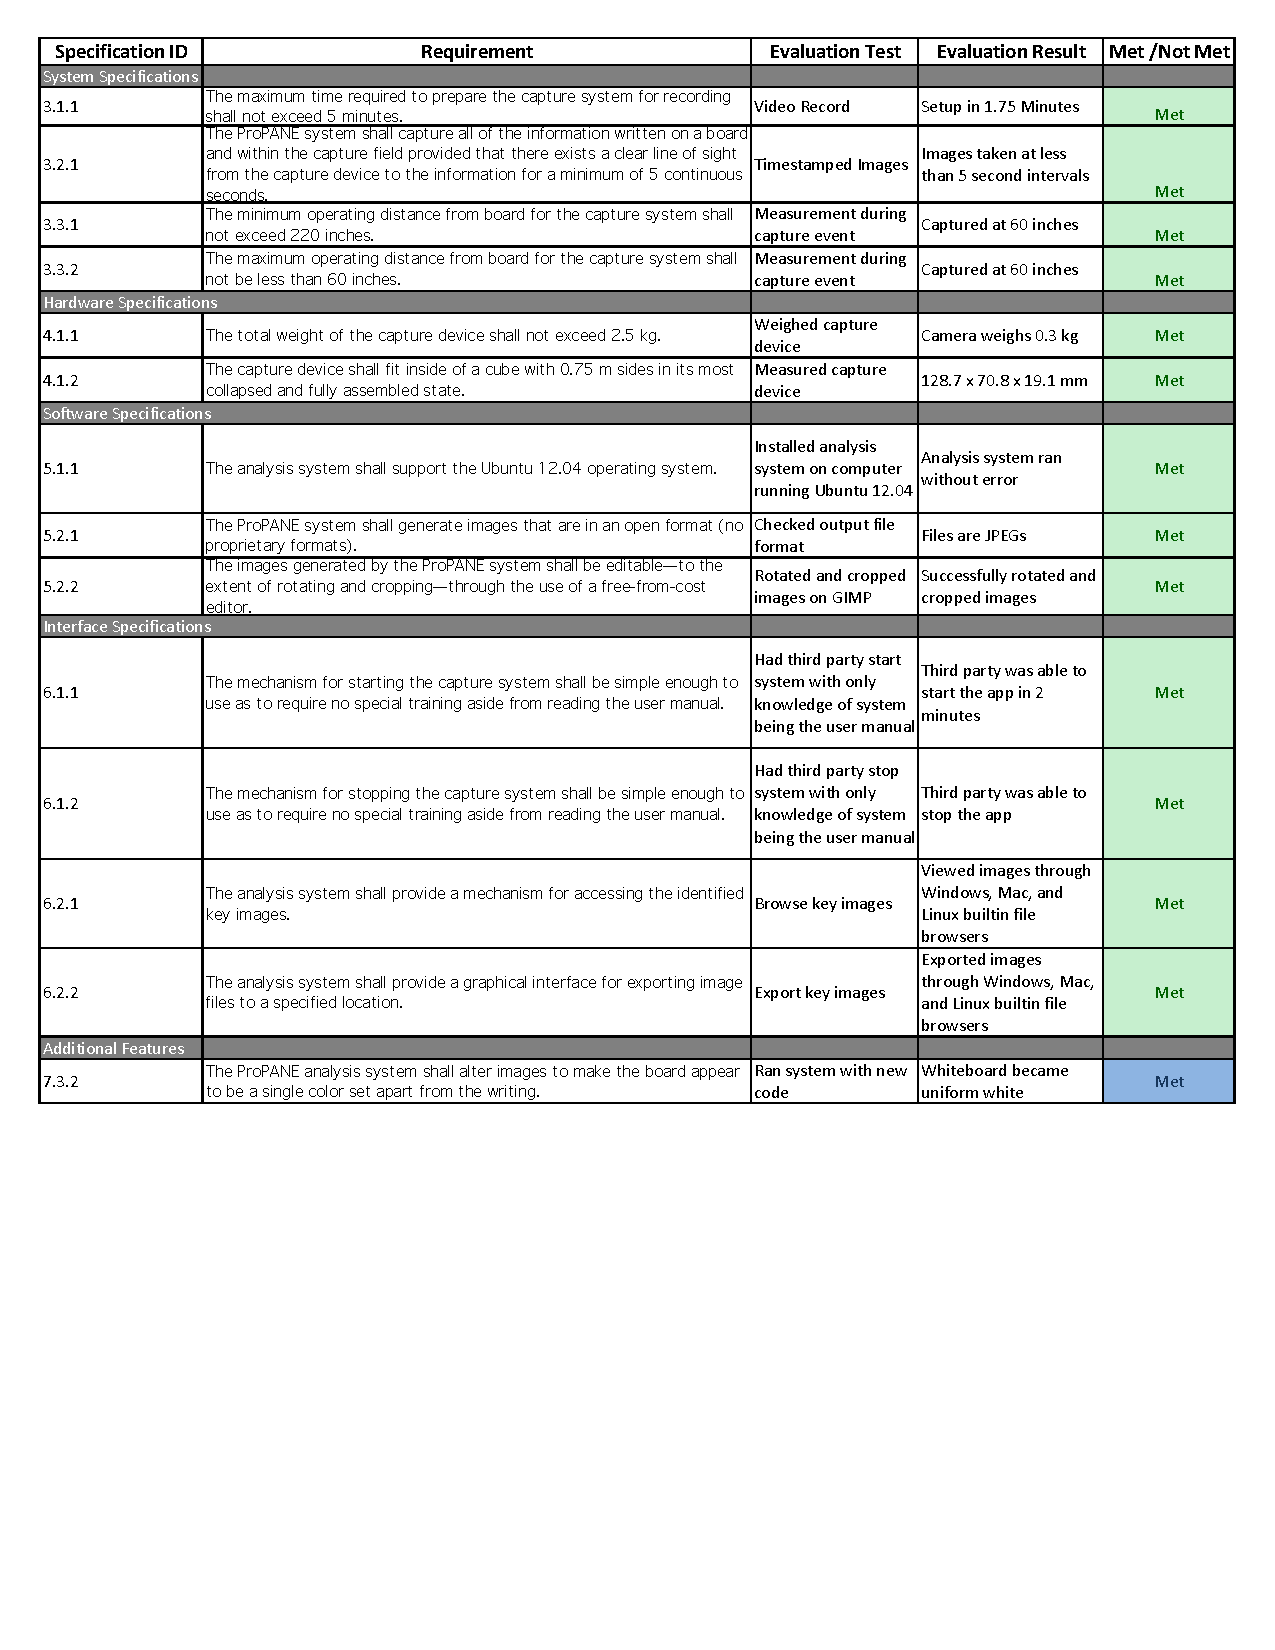
\includegraphics[scale=0.78]{images/technicalspecificationreview.pdf}	
				\caption{Table showing that all technical specifications for this project have been met. Additionally, there is an extra feature (color normalization) that was implemented and tested for the system.}	
				\label{fig:specreview}
			\end{figure}
			
		\subsection{Adjustments to Specifications}
			Specification 5.1.1 was altered from supporting Ubuntu 10.04 to supporting Ubuntu 12.04. This adjustment was made to allow for easier installation of required software for the analysis system. These pieces of software are listed below:
			\begin{itemize}
				\item NumPy
				\item SciPy
				\item Samba Server
			\end{itemize}
			
		\subsection{Additional Specifications Looking Back}
			If we did this project again, we would add the following specifications for how the system should function:
			\begin{itemize}
				\item A key image shall be generated when at least 5\% of all writing on the board and within the capture field has changed or been erased.
				\item The system shall be capable of capturing all information written on a board with dimensions 6 feet by 4 feet.
			\end{itemize}
			The first requirement would be used to ensure that the system is actually generating key images correctly. The second requirement would be used to ensure that the system is actually capturing a usable amount of board space.
					
	\section{Design Evolution}
		
		\subsection{System Architecture}
			The high level view of the system is depicted in Figure \ref{img:concept-of-operation}. The system in broken down into the following three subsystems:
			\begin{itemize}
				\item Capture System: responsible for capturing images of the whiteboard
				\item Analysis System: responsible for processing the images from the capture system
				\item Backend System: responsible for detecting new capture sets and file system manipulations
			\end{itemize}
			\\
			Each of these subsystems is discussed in greater detail in the following sections of the document. 
			
			\begin{figure}[h]
				\centering
				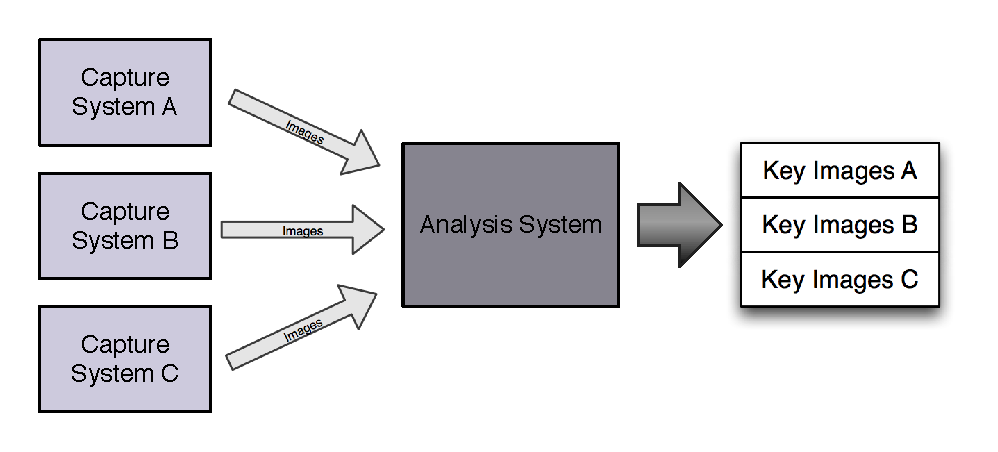
\includegraphics[scale=0.8]{images/concept-of-operation.eps}
				\caption{This figure shows the high level concept of operation where capture systems feed images into the analysis system, which then produces a set of key images. There is a one-to-one relationship between a capture set and a set of key images.}		
				\label{img:concept-of-operation}
			\end{figure}
			
		\subsection{Capture System}
			The requirements from the technical specifications that the capture system had to meet are listed below:
			\begin{itemize}
				\item The maximum time required to prepare the capture system for recording shall not exceed 5 minutes.
				\item The ProPANE system shall capture all of the information written on a board and within the capture field provided that there exists a clear line of sight from the capture device to the information for a minimum of 5 continuous seconds.
				\item The total weight of the capture device shall not exceed 2.5 kg.
				\item The capture device shall fit inside of a cube with 0.75 m sides in its most collapsed and fully assembled state. 
			\end{itemize}
		
		\subsection{Analysis System}
		
		\subsection{Backend System}

	
	\newpage
	\bibliographystyle{ieeetr}
	\bibliography{bibl}
\end{document}